\documentclass{article}

\usepackage[letterpaper,top=1.5cm,bottom=1.5cm,left=2cm,right=2cm,marginparwidth=1.75cm]{geometry}

\usepackage{graphicx}
\usepackage{booktabs}
\usepackage{float} 
\usepackage[colorlinks=true, allcolors=blue]{hyperref}
\usepackage[format=hang,font=small]{caption}

\title{Developing a Model for a Robust and Adaptive Biological Circuit}
\author{Olivia Fernflores}
\date{October 20, 2024}

\begin{document}
\maketitle

\section{Introduction}
Biochemical circuits are essential for modulating signal response in cells. As with any circuit, the topology of the biochemical circuit determines how it responds to different signals. Some motifs are robust to changes in one or many parameters, whereas other motifs only function under a specific set of parameters. Biologically, it important for a signaling system to be able to respond to an input signal by changing the output of a specific protein. Specifically, this paper is concerned with perfect adaptation, which is when a circuit has the ability to rapidly respond to a change in the input signal before quickly returning to some equilibrium concentration. Examples of minimally adaptive circuits are presetned in the paper Ma et al. \cite{challenge2paperD2L} and we seek to find a more robust circuit design. Because we are concerned with biological concentrations of enzymes and proteins and understand that there may be small psychiological changes in parameters that we assume mathematically to be exact numbers, it is important to model circuits that not only respond to the input signal but are also robust to changes in parameter values. By robust to changes in parameter values, we mean that changing one parameter with all else held constant will not render the circuit unable to adapt, which in this paper we classify as a difference in concentrations before and after the response that's less than 10\%. Here, we examine the behavior of the negative feedback loop with a buffer node (NFLBN) presented in Ma et al. \cite{challenge2paperD2L} and find that adding a node and adding a direct relationship between the input response node and the buffer node improves behavioral robustness in response to varrying parameters. 

\section{Model Development}

\subsection{Negative Feedback Loop with a Buffer Node - NFLBN}

The first model for a minimally adaptive biochemical circuit is the model presented of a negative feedback loop with a buffer node presented in \cite{challenge2paperD2L}. As shown in Figure 1, this model has three nodes, A, B, and C. \textit{A} is regulated by the input signal and an enzyme responsible for it's degredation, \textit{Faa}. \textit{B} is degraded by an enzyme, \textit{Fbb}, and is part of negative feedback loop with \textit{C}. \textit{C} controls the output signal, so we look at adaptation in terms of the change in \textit{C} with respect to time.   

\begin{figure}[H]
    \centering
    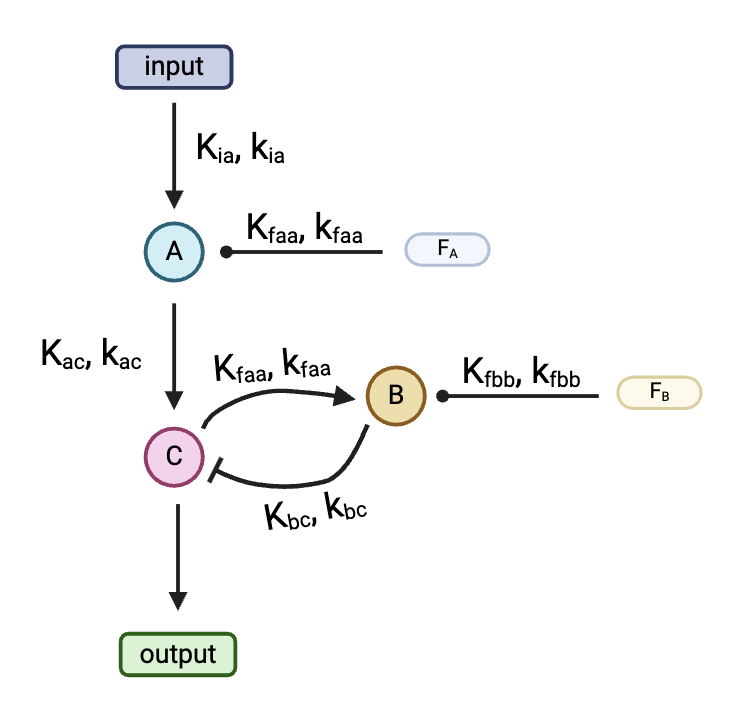
\includegraphics[width=0.7\textwidth]{/Users/olivia/Documents/Fall 2024/MCB 580/MCB580_Challenge2/report/negative_feedback.png}
    \caption{Negative Feedback Loop with a Buffer Node: \textit{A} responds directly to the input signal and is degraded by \textit{Faa}. \textit{B} is activated by \textit{C} and degraded by \textit{Fbb}. \textit{C} activates \textit{B} and is repressed by \textit{B} through a negative feedback loop. \textit{C} also controls the output signal.}
    \label{fig:1}
\end{figure}

The NFLBN can be represented with a set of coupled differential equations modeling enzyme kinetics. As labeled in Figure 1, each node is controlled by two parameters. \textit{K}'s represent the Michaelis-Menten constants named as follows: First enzyme or protein + activates or inhibits + second enzyme or protein. \textit{k}'s represent rate constants describing the speed of each reaction. \textit{Faa} and \textit{Fbb} are initial concentrations of enzymes, and \textit{I} is the strength of the input singal. For an activation process, the Michaelis-Menten equation takes the form 

\[
v = \frac{V_{\max} [S]}{K_m + [S]}
\]


where:
\begin{itemize}
    \item \(v\) is the rate of the reaction (speed per unit time), 
    \item \(V_{\max}\) is the maximum rate (\textit{k} * concentration(s) that affect rate),
    \item \([S]\) is the substrate concentration,
    \item \(K_m\) is the Michaelis-Menten constant.
\end{itemize}



Using this general equation, we can construct a differential equation representing the change in concentration of each node in our circuit with respect to time. Using node \textit{A} as an example, our equation will have two parts:
\\

1. Describes the production of A

\[
\text{I} \cdot k_{ia} \cdot \frac{(1 - A)}{(1 - A) + K_{ia}}
\]


where:
\begin{itemize}
    \item \(\text{I}\) is the strength of the input signal,
    \item \(k_{ia}\) is the rate constant for the input signal's effect on \textit{A},
    \item \((1 - A)\) indicates the available capacity of \textit{A} for production,
    \item \(K_{ia}\) is the Michaelis-Menten constant for production of \textit{A}.
\end{itemize}
\\
2. Describes the degradation of A

\[
F_a \cdot k_{faa} \cdot \frac{A}{A + K_{faa}}
\]

where:
\begin{itemize}
    \item \(F_a\) is concentration of the enzyme that does the reverse reaction (degradation) on \textit{A},
    \item \(k_{faa}\) is the rate constant for the effect of \textit{A} on the consumption of \textit{A},
    \item \(A\) is the concentration of substance \textit{A}in the system,
    \item \(K_{faa}\) is the Michaelis-Menten constant for the degradation of \textit{A}.
\end{itemize}



If you follow this process for all three nodes in the circuit, \textit{A}, \textit{B}, and \textit{C}, you end up with a set of coupled differential equations describing the behavior of the circuit with respect to time. These equations describe concentrations of \textit{A} (1), \textit{B} (2), and \textit{C} (3), and can be solved to model the behavior of the system as parameter values change. 
\\
\\
(1)
\[
\frac{dA}{dt} = \text{I} \cdot k_{ia} \cdot \frac{(1 - A)}{(1 - A) + K_{ia}} - F_a \cdot k_{faa} \cdot \frac{A}{A + K_{faa}}
\]
\\
(2)
\[
\frac{dB}{dt} = C \cdot k_{cb} \cdot \frac{(1 - B)}{(1 - B) + K_{cb}} - F_b \cdot k_{fbb} \cdot \frac{B}{B + K_{fbb}}
\]
\\
(3)
\[
\frac{dC}{dt} = A \cdot k_{ac} \cdot \frac{(1 - C)}{(1 - C) + K_{ac}} - B \cdot k_{bc} \cdot \frac{C}{C + K_{bc}}
\]

Although this circuit is capable of adaptation under specific parameter values, it displays limited robustness to changes in specific parameters. To attempt to make the circuit more robust to parameter changes, we explored adding a node, \textit{D}, to the circuit and incorporating an additional relationship between \textit{A} and \textit{B}. 

\subsection{NFLBN + An Additional Node \textit{D}}

Inspired by the high prevelance of redundancy in biological systems, we decided to add an additional node to our circuit and see if that improved its robustness. Redundancy is frequently used biologically to allow robustness, such as gene duplications for genes with critical functions, multiple types of immune system responses that ensure a response even when part of the system fails, and pathways during limb development that serve the same function but are controlled differently. In our model, we incorporate a fourth node, \textit{D}, that also regulates \textit{C} through a negative feedback loop, but the relationship is reverse to that of \textit{B} and \textit{C}. This isn't completely redundant to the relationship between \textit{B} and \textit{C}, but it is a more interesting case to explore because it is not the same as the existing circuit. As seen in Figure 2, most of the circuit is unchanged, so our equations for \textit{A} and \textit{B} will stay the same. 
\\
\\
(1)
\[
\frac{dA}{dt} = \text{I} \cdot k_{ia} \cdot \frac{(1 - A)}{(1 - A) + K_{ia}} - F_a \cdot k_{faa} \cdot \frac{A}{A + K_{faa}}
\]
\\
(2)
\[
\frac{dB}{dt} = C \cdot k_{cb} \cdot \frac{(1 - B)}{(1 - B) + K_{cb}} - F_b \cdot k_{fbb} \cdot \frac{B}{B + K_{fbb}}
\]
\\

When it comes to \textit{C}, our equation will incorporate an additional term to describe its activation by C. Using the same technique described for the NFLBN model, this yields the following equation for \textit{C}:
\\
\\
(3)
\[
\frac{dC}{dt} = A \cdot k_{ac} \cdot \frac{(1 - C)}{(1 - C) + K_{ac}} - B \cdot k_{bc} \cdot \frac{C}{C + K_{bc}} + D \cdot k_{cd} \cdot \frac{(1 - C)}{(1 - C) + K_{dc}}
\]

Because we now have a fourth node in our system, we must also add a fourth differential equation to represent the concentration of this species. \textit{D} is activated by \textit{A}, and degraded by both \textit{Fd} and \textit{C}. Our equation will have three terms, one for production of \textit{D} by \textit{A}, and two for degradtion by each of \textit{Fd} and \textit{C}. Overall, this gives the following equation:
\\
\\
(4)
\[
\frac{dD}{dt} = A \cdot k_{ad} \cdot \frac{(1 - D)}{(1 - D) + K_{ad}} - F_d \cdot k_{fdd} \cdot \frac{D}{D + K_{fdd}} - C \cdot k_{cd} \cdot \frac{D}{D + K_{cd}}
\]

Together, these equations represent the system described and shown in Figure 2. 

\begin{figure}[H]
    \centering
    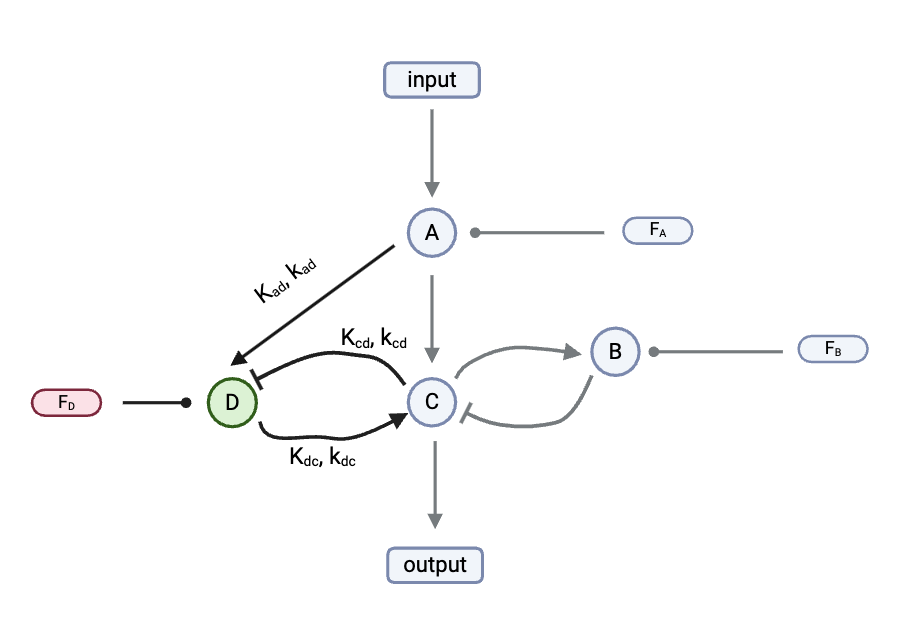
\includegraphics[width=0.7\textwidth]{/Users/olivia/Documents/Fall 2024/MCB 580/MCB580_Challenge2/report/negative_feedback_add_D.png}
    \caption{NFLBN + Additional Node \textid{D}: New components of the circuit added to this model are shown in color. The only new relationships are \textit{A} activating \textit{D}, and the feedback loop between \textit{C} and \textit{D}.}
    \label{fig:2}
\end{figure}

\subsection{NFLBN + An Additional Node \textit{D} + Direct Relationship Between \textit{A} and \textit{B}}

The final model we considered in this paper builds on the previous model where we added node \textit{D} and incorporates a direct relationship between the input response node, \textit{A}, and the buffer node, \textit{B}. As shown in Figure 3, we took previous model of NFLBN + Node \textit{D} and added complexity by allowing \textit{A} to directly inhibit \textit{B}. 

\begin{figure}[H]
    \centering
    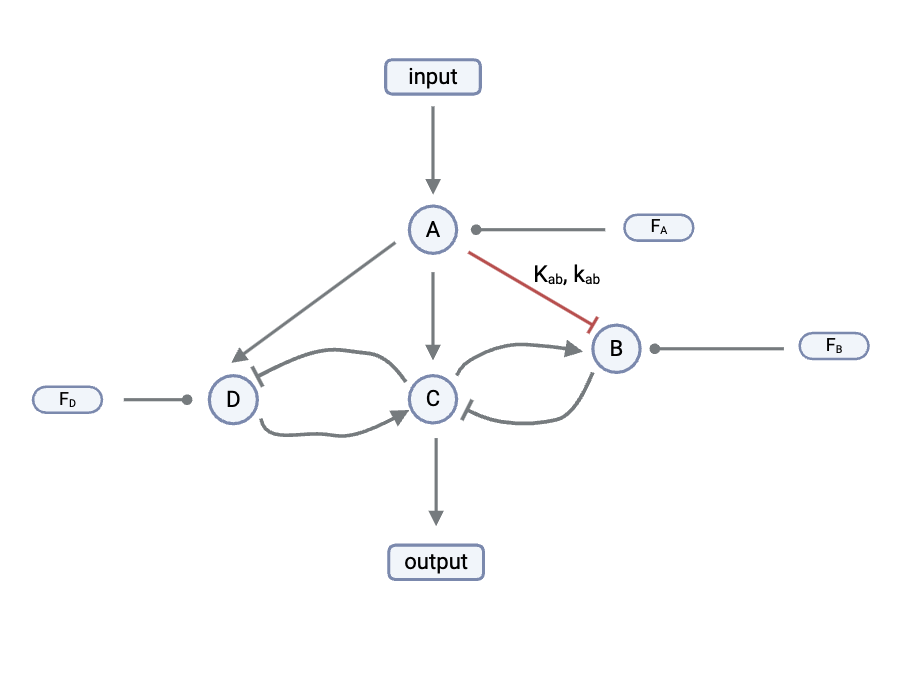
\includegraphics[width=0.7\textwidth]{/Users/olivia/Documents/Fall 2024/MCB 580/MCB580_Challenge2/report/negative_feedback_add_D_and_A_regulates_B.png}
    \caption{NFLBN + Additional Node \textid{D}: New components of the circuit added to this model are shown in red. The only new relationships is \textit{A} inhibiting \textit{B}.}
    \label{fig:3}
\end{figure}

This is the most complex model we explored in this paper. Because there is only one difference between this model and the previous model, and that change only applies to \textit{B}, we need to update the equation describing the change in \textit{B} over time to include a term for its inhibition by \textit{A}. Again, using the same principles for constructing Michaelis-Menten equations described earlier, we must add the term
\\

\[A \cdot k_{ab} \cdot \frac{B}{B + K_{ab}}\]

\\
\\
\\
This gives the following equation for \textit{B}:

\\
\[
\frac{dB}{dt} = C \cdot k_{cb} \cdot \frac{(1 - B)}{(1 - B) + K_{cb}} - F_b \cdot k_{fbb} \cdot \frac{B}{B + K_{fbb}} - A \cdot k_{ab} \cdot \frac{B}{B + K_{ab}}
\]
\\
\\

Using this equation in place of equation 2 as previously described, our circuit can be modeled by these four equations. 
\\
\\
(1)
\[
\frac{dA}{dt} = \text{I} \cdot k_{ia} \cdot \frac{(1 - A)}{(1 - A) + K_{ia}} - F_a \cdot k_{faa} \cdot \frac{A}{A + K_{faa}}
\]
\\
(2)
\[
\frac{dB}{dt} = C \cdot k_{cb} \cdot \frac{(1 - B)}{(1 - B) + K_{cb}} - F_b \cdot k_{fbb} \cdot \frac{B}{B + K_{fbb}} - A \cdot k_{ab} \cdot \frac{B}{B + K_{ab}}
\]
\\
(3)
\[
\frac{dC}{dt} = A \cdot k_{ac} \cdot \frac{(1 - C)}{(1 - C) + K_{ac}} - B \cdot k_{bc} \cdot \frac{C}{C + K_{bc}} + D \cdot k_{cd} \cdot \frac{(1 - C)}{(1 - C) + K_{dc}}
\]
\\
(4)
\[
\frac{dD}{dt} = A \cdot k_{ad} \cdot \frac{(1 - D)}{(1 - D) + K_{ad}} - F_d \cdot k_{fdd} \cdot \frac{D}{D + K_{fdd}} - C \cdot k_{cd} \cdot \frac{D}{D + K_{cd}}
\]
\\

\section{Results}

\subsection{Finding Parameter Values for the NFLBN that Allow Adaptation}

The first step in this project was to find a set of parameter values that allow the NFLBN to behave adaptively in response to an input signal. Using the guidelines in Ma et al. \cite{challenge2paperD2L}, we did a parameter sweep across powers of 10 from $1 \times 10^{-2}$ to $1 \times 10^{2}$ using initial concentrations of 0.1, 0.1, and 0.5 for \textit{A}, \textit{B}, and \textit{C} respectively and initial input singal strength of 1 (beginning), adding signal (input = 2) and removing signal (input = 1) every 200 time units (green and red lines on the plot). Iteratively, we examined the behavior of the circuit as we varried each of 13 parameters in our differentials equations while keeping the rest constant. An example of some of the plots generated from these parameter sweeps can be seen below in Figure 4 and the parameter values that allow the NFLBN circuit to behave adaptively are shown in Table 1 (called ``Adaptive Parameters'' for the remainder of the paper). 

\begin{figure}[H]
    \centering
    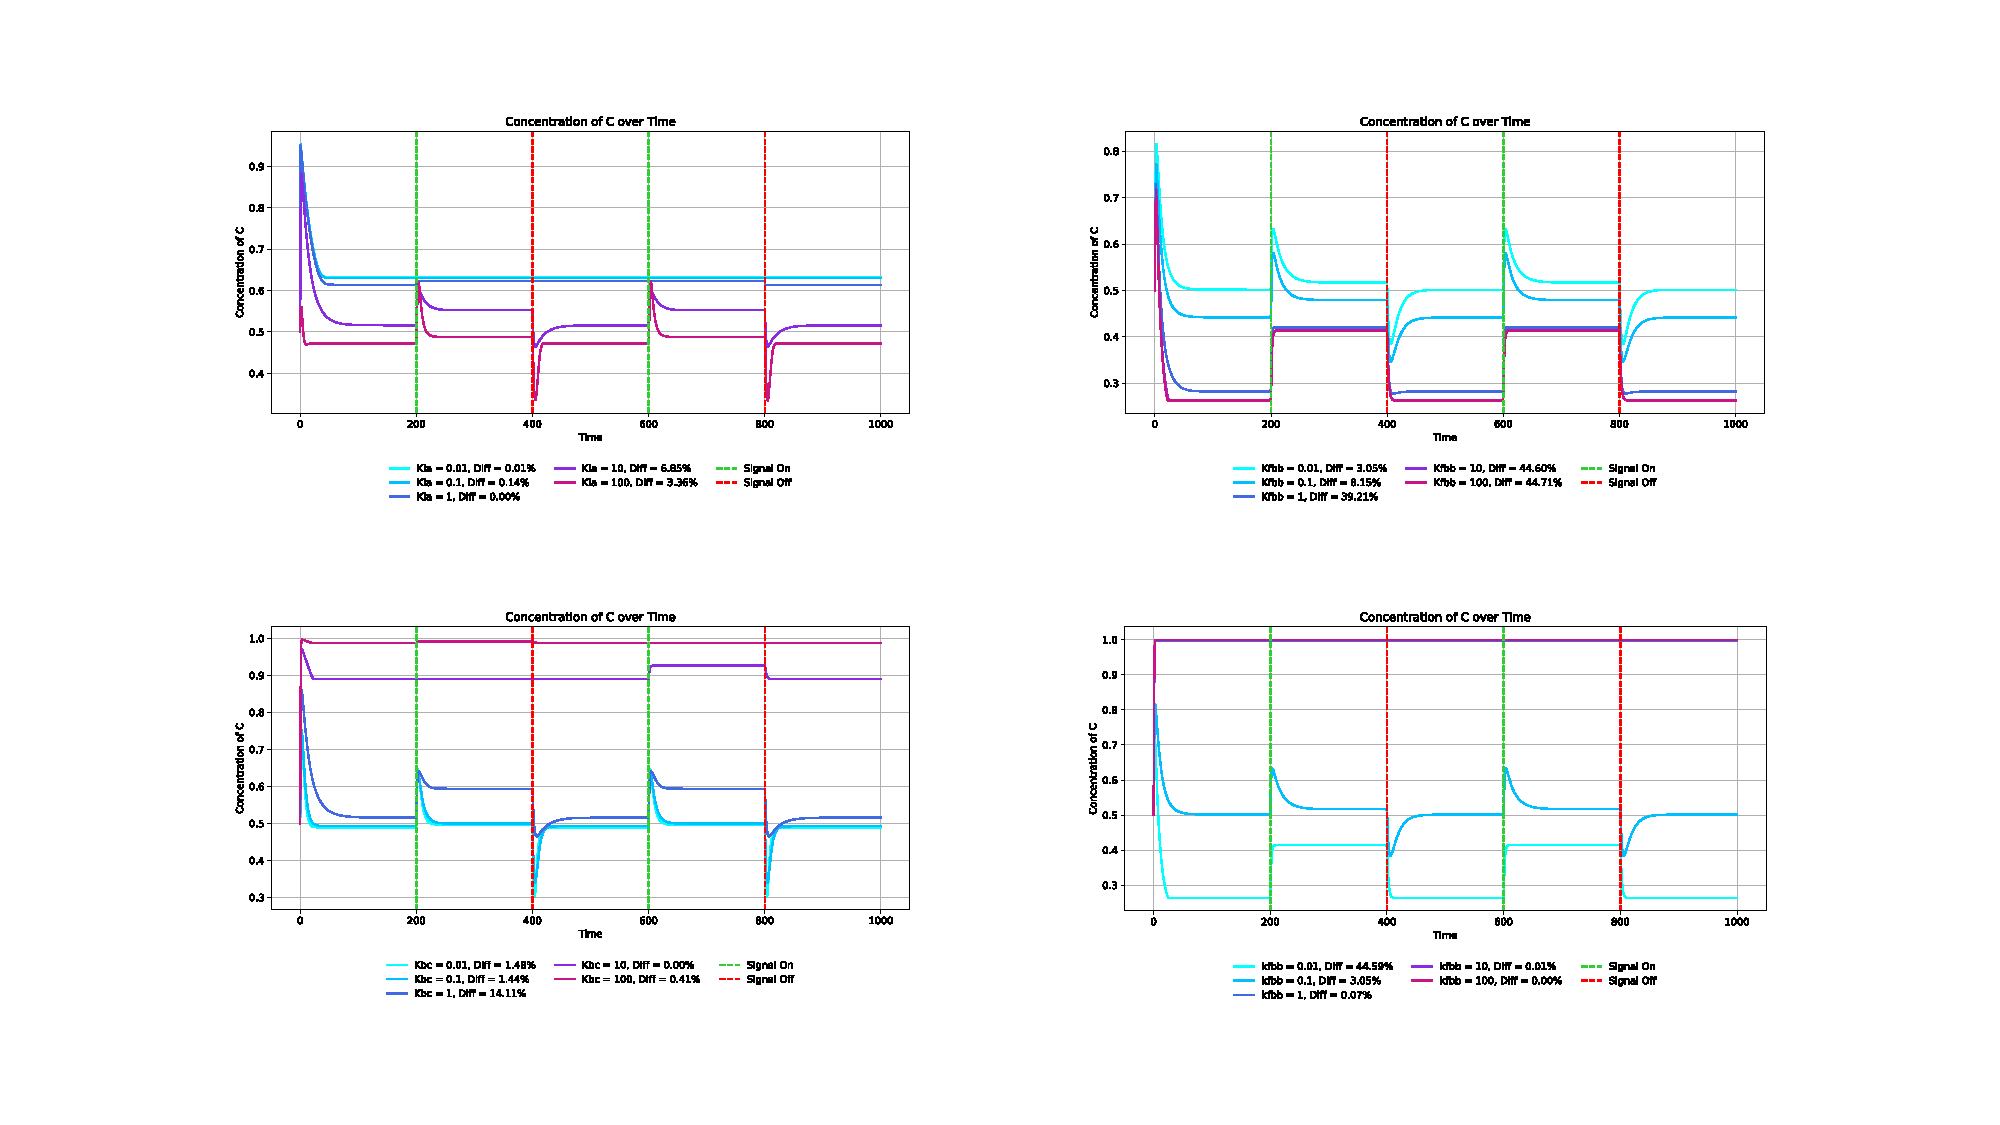
\includegraphics[width=0.7\textwidth]{/Users/olivia/Documents/Fall 2024/MCB 580/MCB580_Challenge2/report/ParameterSweepExample.pdf}
    \caption{An example of the parameter sweep results for the NFLBN. Initial concentrations of 0.1, 0.1, and 0.5 for \textit{A}, \textit{B}, and \textit{C} respectively. Input signal begins at 1, changes to 2 at the green dotted line, then goes back to 1 at the red dotted line. This continues every 200 time units. All other parameters held constant.}
    \label{fig:4}
\end{figure}

\begin{table}[h]
    \centering
    \caption{NFLBN Adaptive Behavior Parameters}
    \begin{tabular}{@{}ll@{}}
        \toprule
        Parameter & Value \\ 
        \midrule
        \(k_{ia}\) & 5 \\
        \(K_{ia}\) & 20 \\
        \(F_a\) & 0.5 \\
        \(k_{faa}\) & 1 \\
        \(K_{faa}\) & 1 \\
        \(k_{cb}\) & 0.1 \\
        \(K_{cb}\) & 0.01 \\
        \(F_b\) & 0.5 \\
        \(k_{fbb}\) & 0.1 \\
        \(K_{fbb}\) & 0.01 \\
        \(k_{ac}\) & 10 \\
        \(K_{ac}\) & 1 \\
        \(k_{bc}\) & 5 \\
        \(K_{bc}\) & 0.5 \\
        \bottomrule
    \end{tabular}
    \label{tab:parameters}
\end{table}

The parameters seen in Table 1, concentrations for \textit{A}, \textit{B}, and \textit{C}, and input signal levels are the values used for the remainder of the paper unless specified otherwise. In Figure 5, we plot the concentration of \textit{C} using this set of parameters. This is our basic model and will serve as the comparison for the rest of our models. 

\begin{figure}[H]
    \centering
    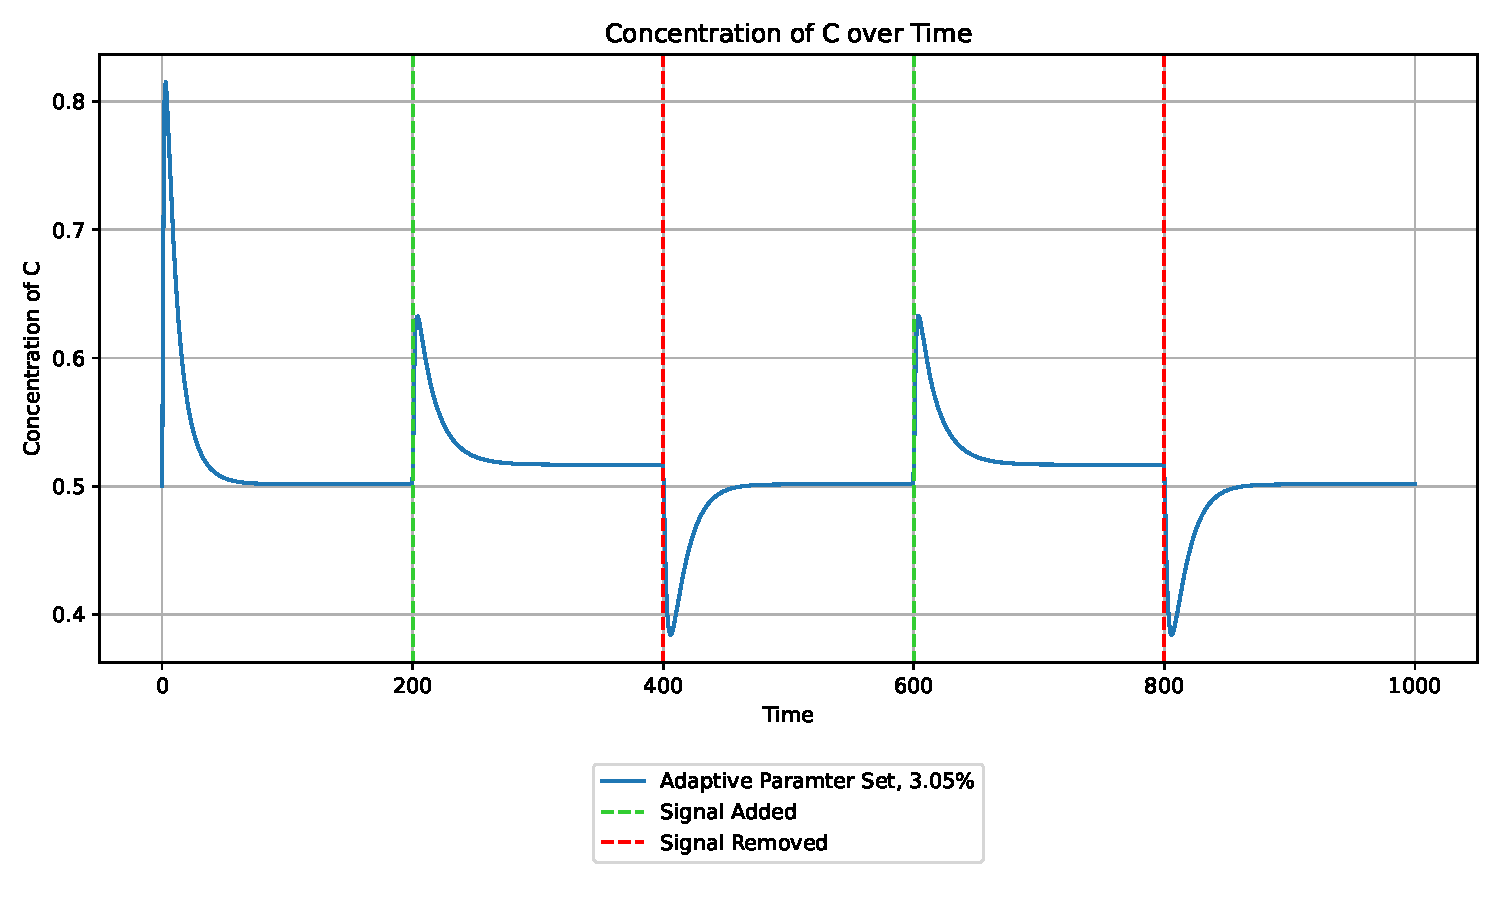
\includegraphics[width=0.7\textwidth]{/Users/olivia/Documents/Fall 2024/MCB 580/MCB580_Challenge2/results/negative_basic_model.pdf}
    \caption{The behavior of the NFLBN circuit under the parameter conditions specified in Table 1. 3.05\% is the difference between the concentration of \textit{C} after responding to a signal increase (green line) and a signal decrease (red line).}
    \label{fig:5}
\end{figure}

\subsection{Adaptation in NFLBN + \textit{D}}

The parameter sweep for the basic model showed that although there are conditions under which the basic model is adaptive, it's very limited. Using our more complex model that incorporates redundancy with an opposite relationship to that of \textit{B} and \textit{C}, we simulated our more complex model, first using the same parameter values that worked for the NFLBN circuit and just adding the values for the new parameters. Quickly, we saw that the more complex model is also adaptive under our adaptive parameters, as illustrated in Figure 6. 

\begin{figure}[H]
    \centering
    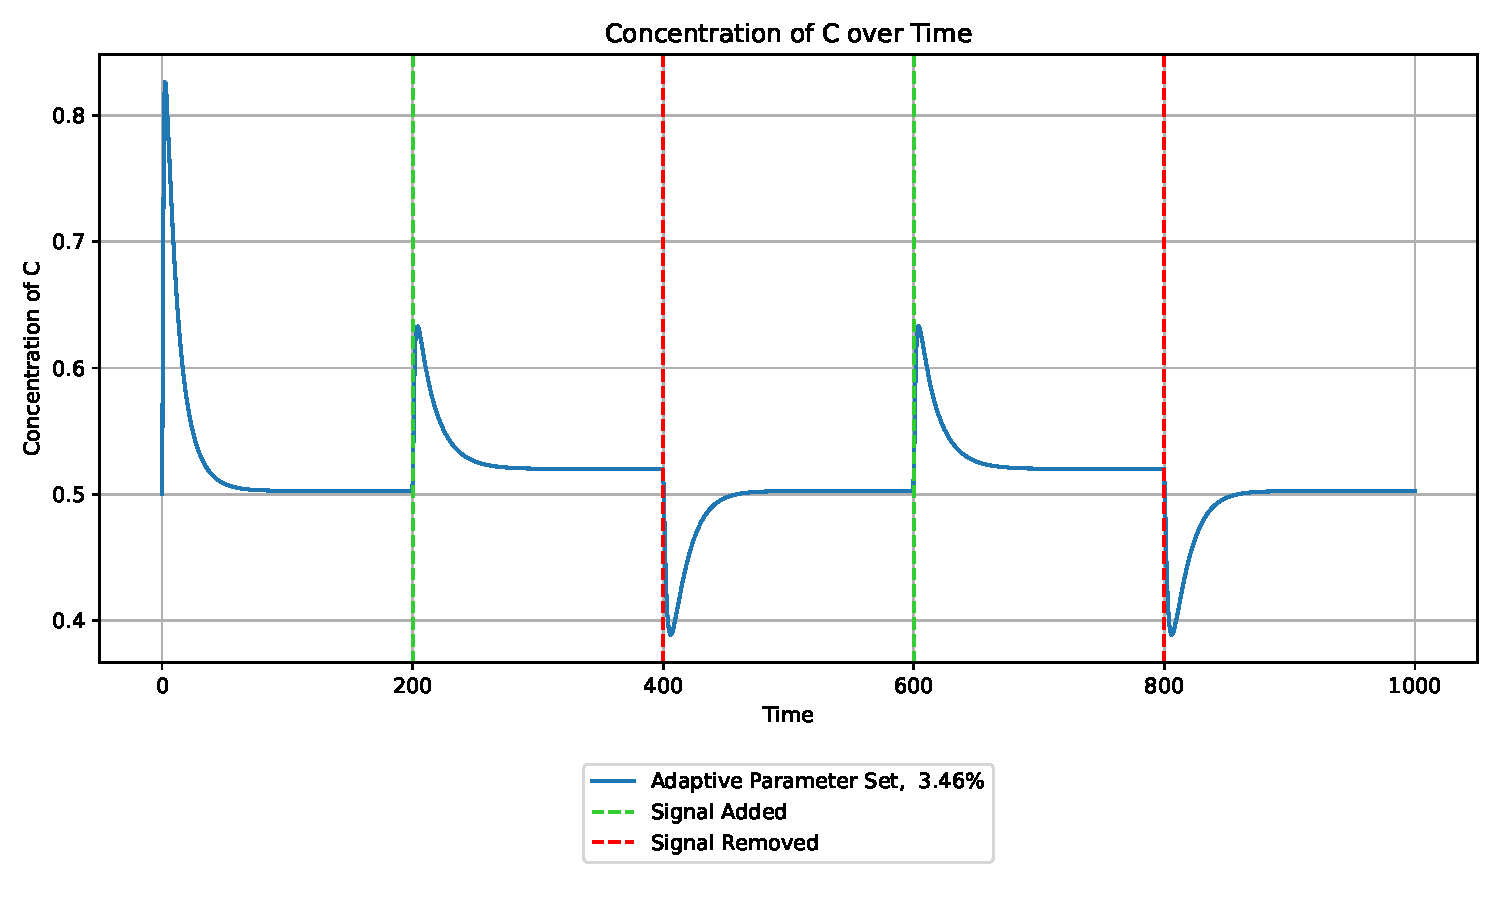
\includegraphics[width=0.7\textwidth]{/Users/olivia/Documents/Fall 2024/MCB 580/MCB580_Challenge2/results/negative_add_D_model.pdf}
    \caption{The behavior of the NFLBN circuit with node \textit{D} added under the parameter conditions specified in Table 1. 3.46\% is the difference between the concentration of \textit{C} after responding to a signal increase (green line) and a signal decrease (red line).}
    \label{fig:6}
\end{figure}

Once we saw that this model was also adaptive under our parameter set, we tested the robustness of this model compared to the NFLBN circuit. Again, using our adaptive parameters set, we perturbed individual parameters holding the rest constant and examined the range under which the circuit still displayed adaptive behavior. Although adding node \textit{D} was not enough to show robustness to parameter changes across all parameters used in the simple NFLBN model, it did significantly improve robustness in response to changes in specific parameters. In Figures 7 and 8, we show the results of varrying \textit{Fa}, \textit{kfaa}, and \textit{kbc}, which the NFLBN + \textit{D} is more robust in changes to compared to the NFLBN model. These findings are summarized in Table 2. 

\begin{figure}[H]
    \centering
    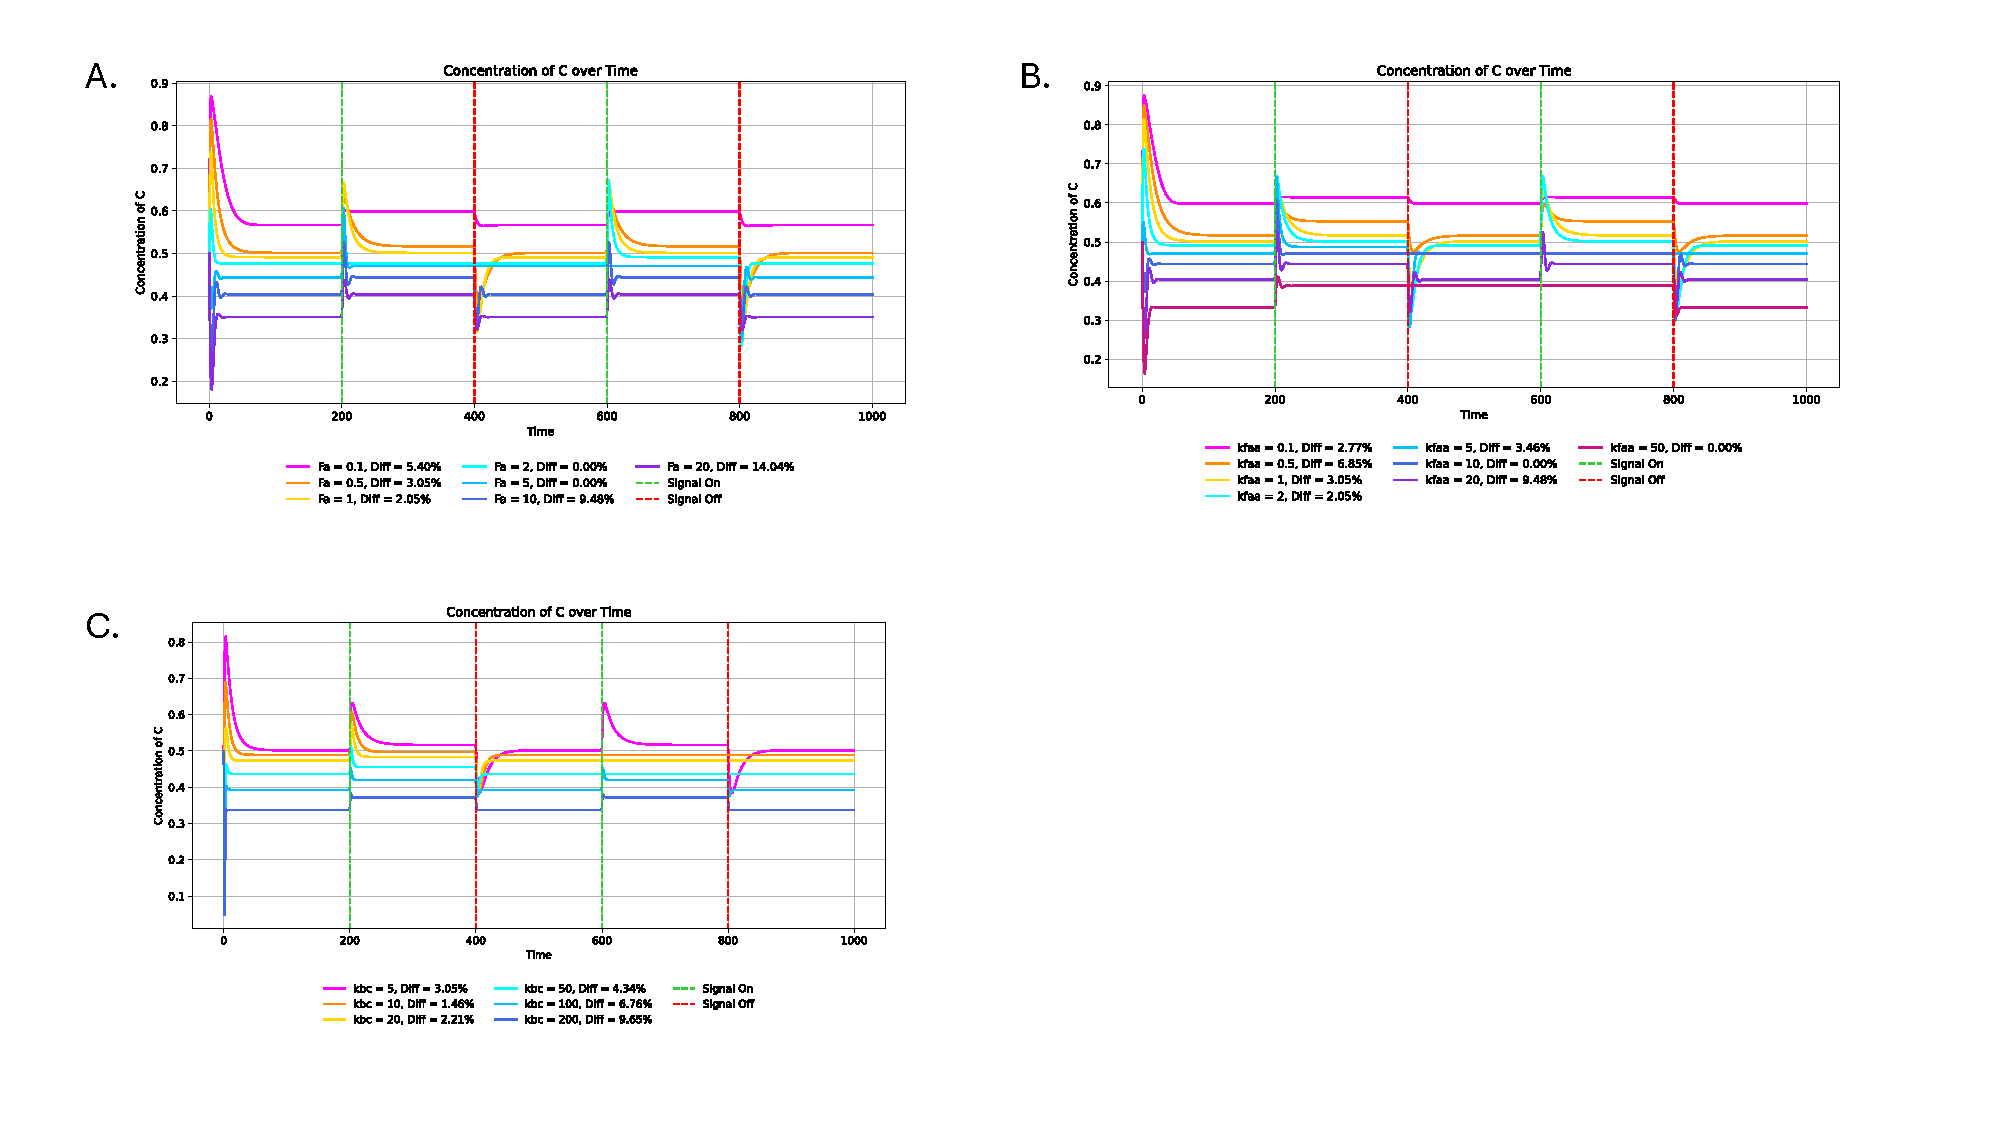
\includegraphics[width=0.7\textwidth]{/Users/olivia/Documents/Fall 2024/MCB 580/MCB580_Challenge2/report/negative_basic_explore_1.pdf}
    \caption{The NFLBN shows limited or no robustness to changes in parameters \textit{Fa}, \textit{kfaa}, and \textit{kbc}. Varrying values for \textit{Fa} (A), \textit{kfaa} (B), and \textit{kcb} (C), with all other parameters set to the adaptive paramater values previously described. Input signal begins at 1, changes to 2 at the green dotted line, then goes back to 1 at the red dotted line. This continues every 200 time units. All other parameters held constant.}
    \label{fig:7}
\end{figure}

\begin{figure}[H]
    \centering
    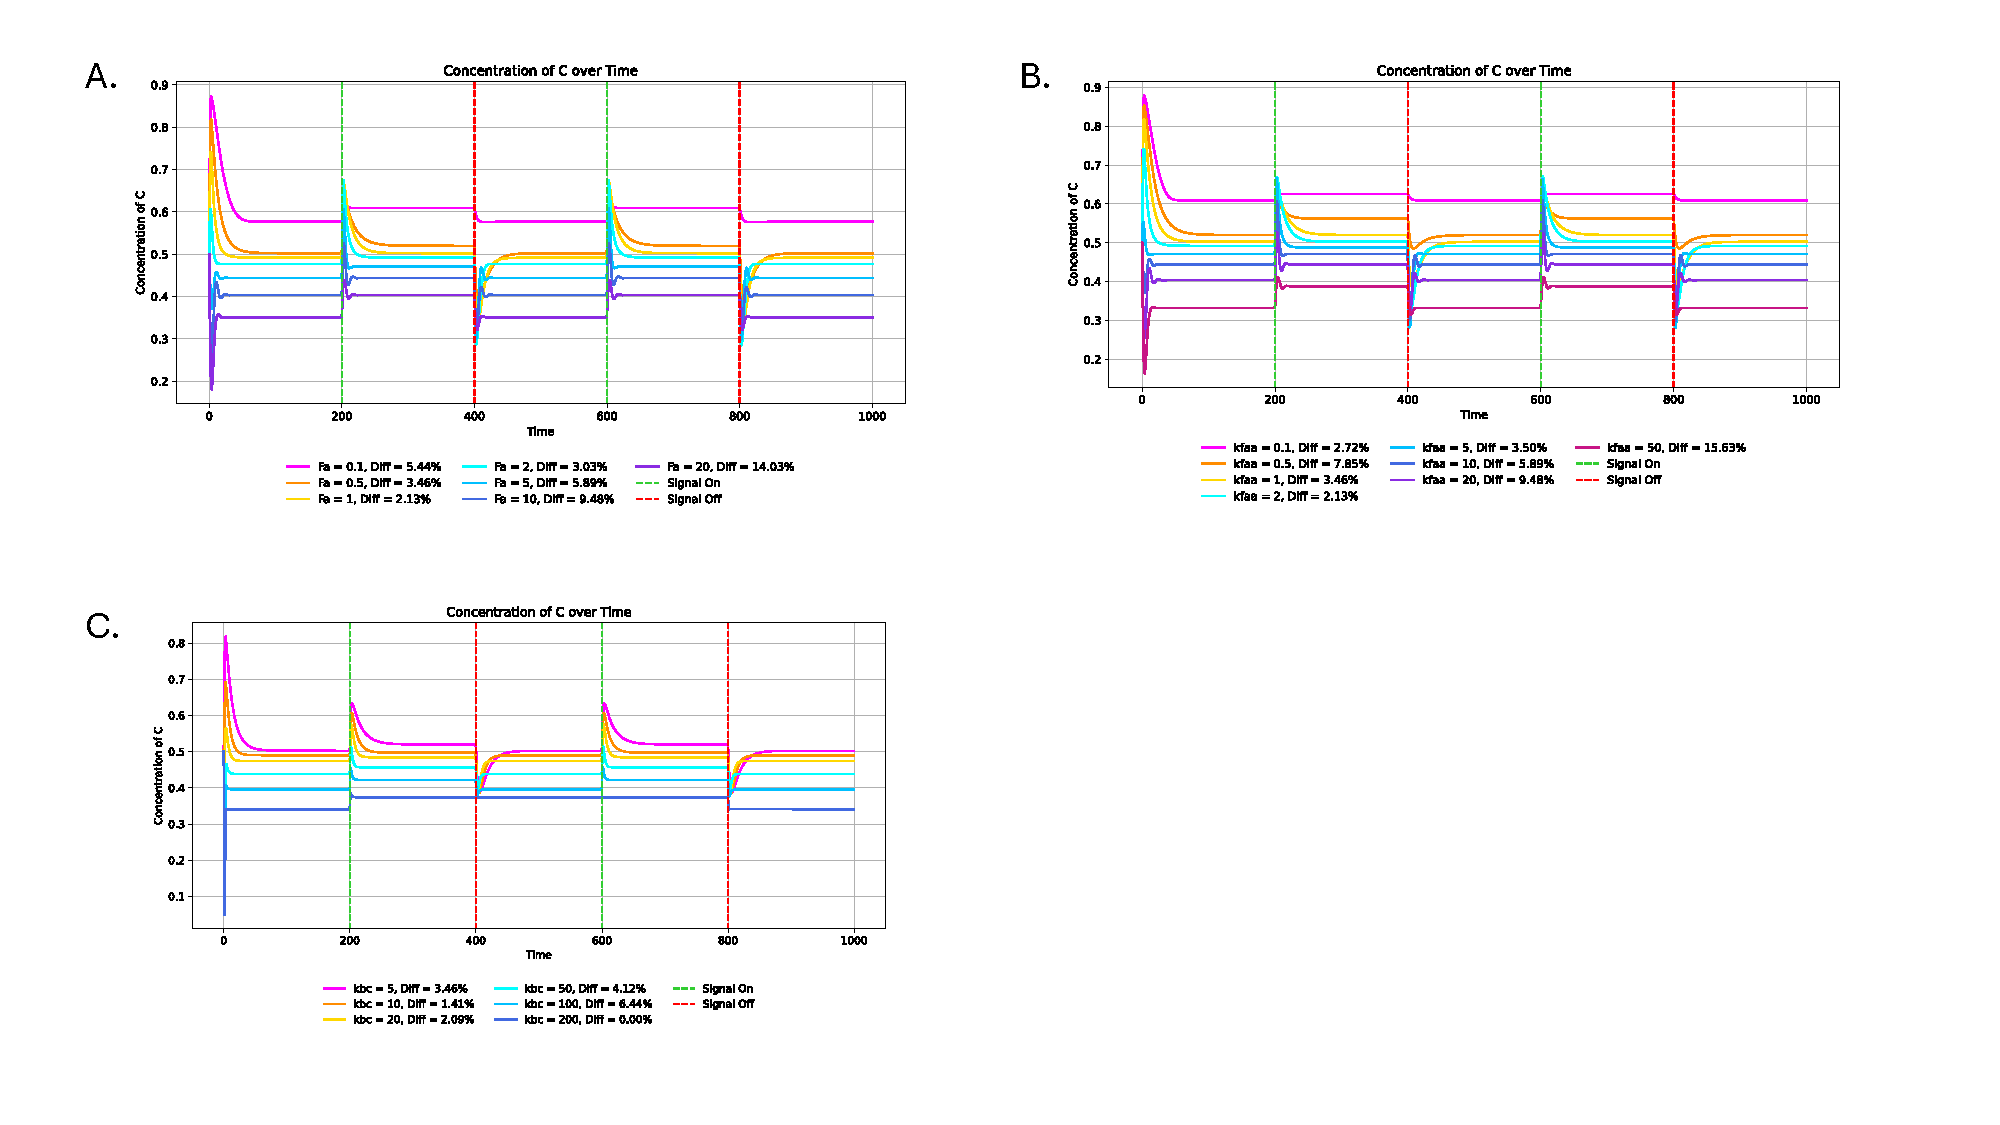
\includegraphics[width=0.7\textwidth]{/Users/olivia/Documents/Fall 2024/MCB 580/MCB580_Challenge2/report/negative_plus_D_explore.pdf}
    \caption{The NFLBN + \textit{D} shows improved robustness to changes in parameters \textit{Fa}, \textit{kfaa}, and \textit{kbc} compared to the NFLBN. Varrying values for \textit{Fa} (A), \textit{kfaa} (B), and \textit{kcb} (C), with all other parameters set to the adaptive paramater values previously described. Input signal begins at 1, changes to 2 at the green dotted line, then goes back to 1 at the red dotted line. This continues every 200 time units. All other parameters held constant.}
    \label{fig:8}
\end{figure}

\begin{table}[h]
    \centering
    \caption{NFLBN and NFLBN + \textit{D} Adaptive Parameter Value Comparison}
    \begin{tabular}{@{}lll@{}}
        \toprule
        Parameter & NFLBN Value & NFLBN + \textit{D} Value\\ 
        \midrule
        \(F_a\) & 0.5, 1 & 0.5, 1, 2, 5\\
        \(k_{faa}\) & 0.5, 1, 2 & 0.5, 1, 2, 5, 10, 20 \\
        \(k_{bc}\) & 5 & 5, 10, 20, 50, 100\\
        \bottomrule
    \end{tabular}
    \label{tab:parameters}
\end{table}

As shown by the values in Table 2, the adaptive behavior of NFLBN + \textit{D} is significant compared to that of the NFLBN. With paramater \textit{Fa}, the NFLBN + \textit{D} can withstand paramater values of a ten-fold difference from 0.5 to 5, whereas the basic NFLBN can only withstand a two-fold difference from 0.5 to 1. For \textit{kfaa}, the basic NFLBN model can continue adaptive behavior under parameters from 0.5 to 2, but the NFLBN + \textit{D} model can behave adaptively from 0.5 to 20, a range that's ten-fold larger in the NFLBN + \textit{D} model. Finally, when it comes to \textit{kbc}, the NFLBN is not robust at all to parameter changes and only behaves adaptively when \textit{kbc = 5}. Contrastingly, the NFLBN + \textit{D} model behaves adaptively with \texitit{kbc} from 5 to 100, showing much greater robustness to parameter changes.

\subsection{Adaptation in NFLBN + \textit{D} + \textit{A} regulates \textit{B}}

Continuing to search for robustness to changes in parameter values, we performed the same simulations for our most complex model that builds on the previous NFLBN + \textit{D} model to also include \textit{A} inhibiting \textit{B}. We found that this new model of NFLBN + \textit{D} + \textit{A} regulates \textit{B} added robustness to parameter changes in \textit{kac}, which was not a parameter space where we saw robustness to change in previous models. As summarized in Table 3, this model could withstand parameters of 1, 2, 5, and 10 for \textit{kac}, which our other models could not achieve. Table 3 also shows that robustness across changes in \textit{Fa}, \textit{kfaa}, and \textit{kbc} remains as it was in the previous model (NFLBN + \textit{D}) and is even improved in the case of \textit{Fa}. 

\begin{table}[h]
    \centering
    \caption{NFLBN, NFLBN + \textit{D}, and NFLBN + \textit{D} + \textit{A} regulates \textit{B} Adaptive Parameter Value Comparison}
    \begin{tabular}{@{}llll@{}}
        \toprule
        Parameter & NFLBN Value & NFLBN + \textit{D} Value & NFLBN + \textit{D} + \textit{A} regulates \textit{B} Value\\ 
        \midrule
        \(F_a\) & 0.5, 1 & 0.5, 1, 2, 5 & 0.5, 1, 2, 5, 10\\
        \(k_{faa}\) & 0.5, 1, 2 & 0.5, 1, 2, 5, 10, 20 & 0.5, 1, 2, 5, 10, 20 \\
        \(k_{bc}\) & 5 & 5, 10, 20, 50, 100 & 5, 10, 20, 50, 100\\
        \(k_{ac}\) & 5, 10 & 1, 5, 10 & 1, 2, 5, 10\\
        \bottomrule
    \end{tabular}
    \label{tab:parameters}
\end{table}

For the simulations summarized in Table 3, as with all simulations throughout the paper, all other parameters were held fixed at their adaptive values (see Table 1), initial concentrations of 0.1, 0.1, and 0.5 were used for \textit{A}, \textit{B}, and \textit{C} respectively. The parameters that were added as model complexity increased were also constant throughout simulations (ex. \textit{kad} in both NFLBN + \textit{D} and NFLBN + \textit{D} + \textit{A} is equal to 1). The following three figures (9-11) show the results of the simulations described above. 

\begin{figure}[H]
    \centering
    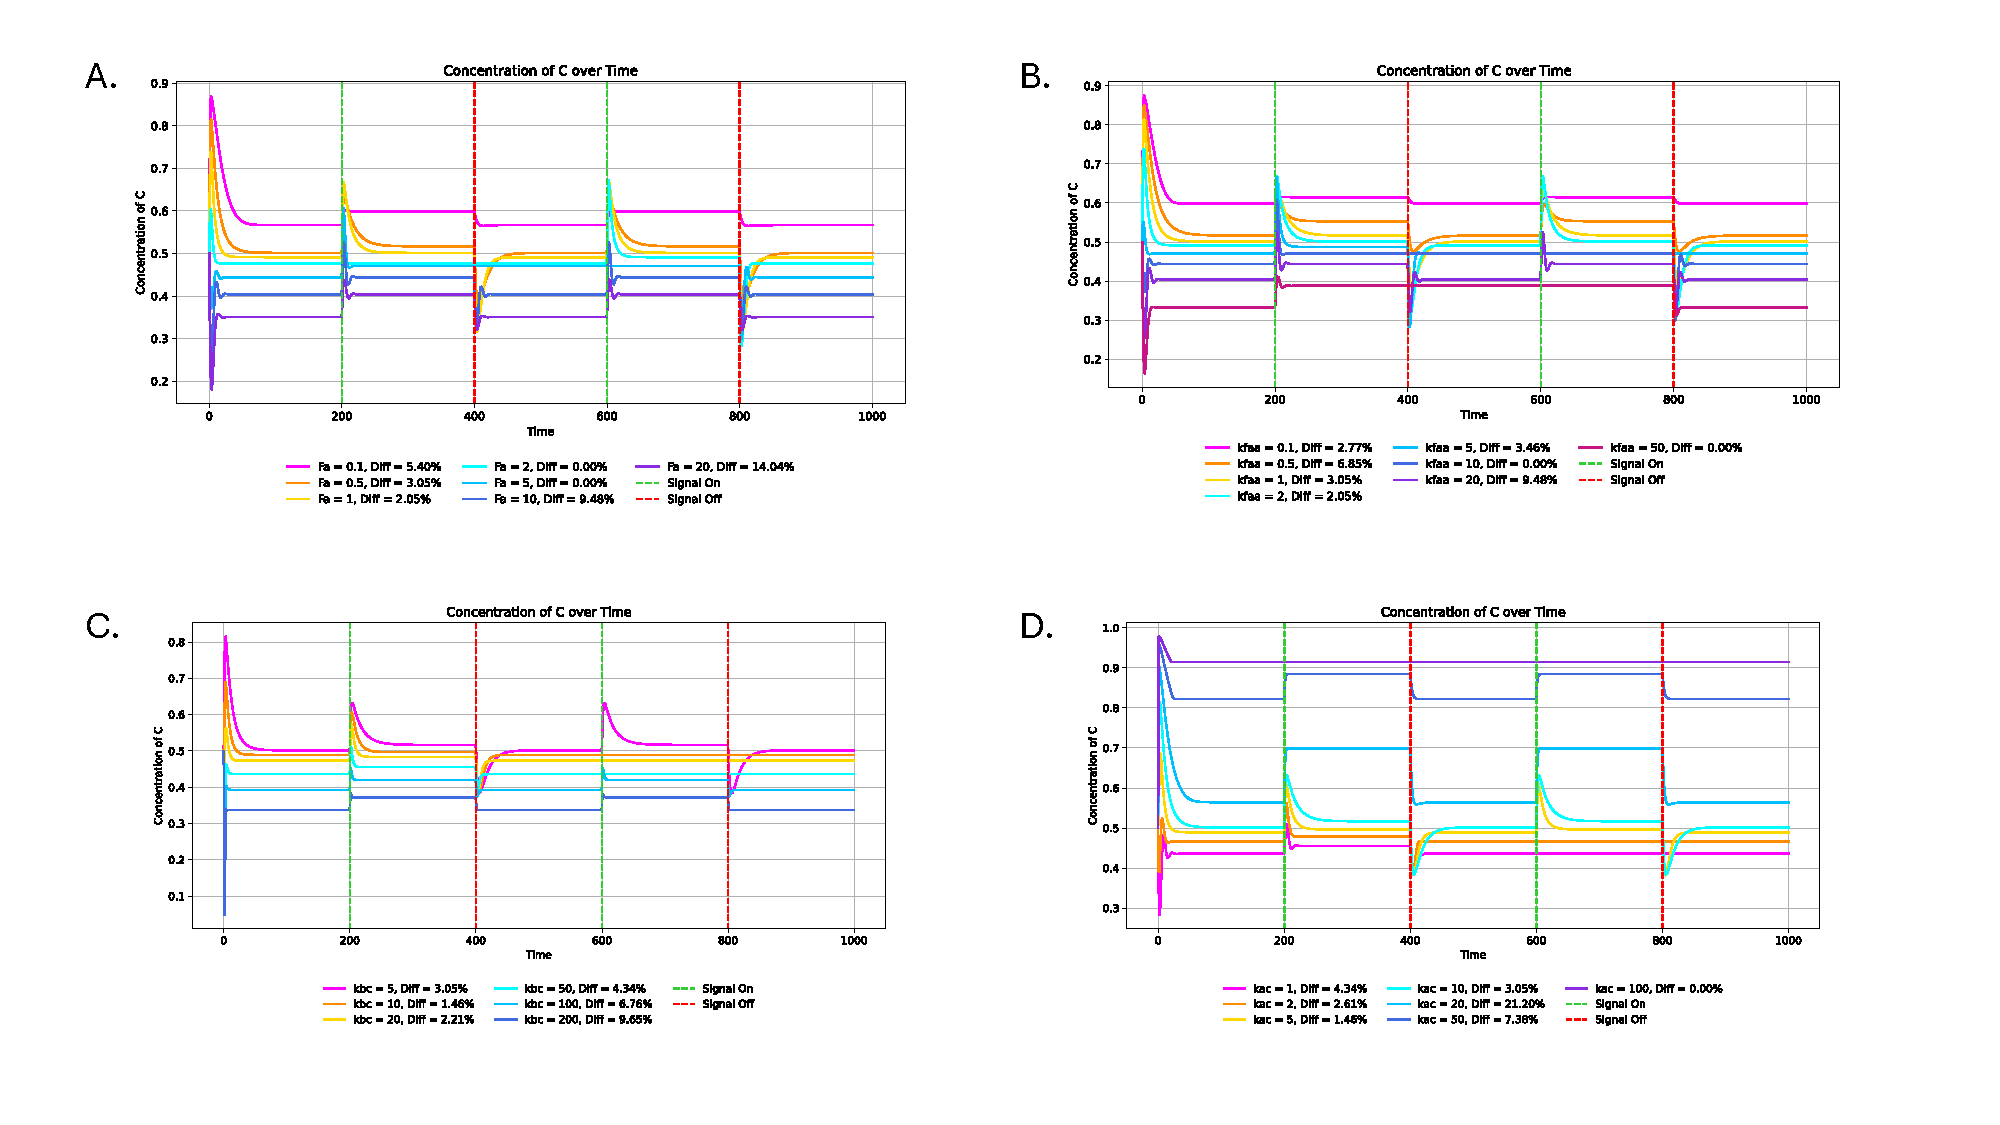
\includegraphics[width=0.7\textwidth]{/Users/olivia/Documents/Fall 2024/MCB 580/MCB580_Challenge2/report/negative_feedback_explore_2.pdf}
    \caption{The NFLBN shows limited or no robustness to changes in parameters \textit{Fa}, \textit{kfaa}, \textit{kbc}, and \textit{kac}. Varrying values for \textit{Fa} (A), \textit{kfaa} (B), and \textit{kcb} (C), and \textit{kac} (D), with all other parameters set to the adaptive paramater values previously described. Input signal begins at 1, changes to 2 at the green dotted line, then goes back to 1 at the red dotted line. This continues every 200 time units. All other parameters held constant.}
    \label{fig:9}
\end{figure}

\begin{figure}[H]
    \centering
    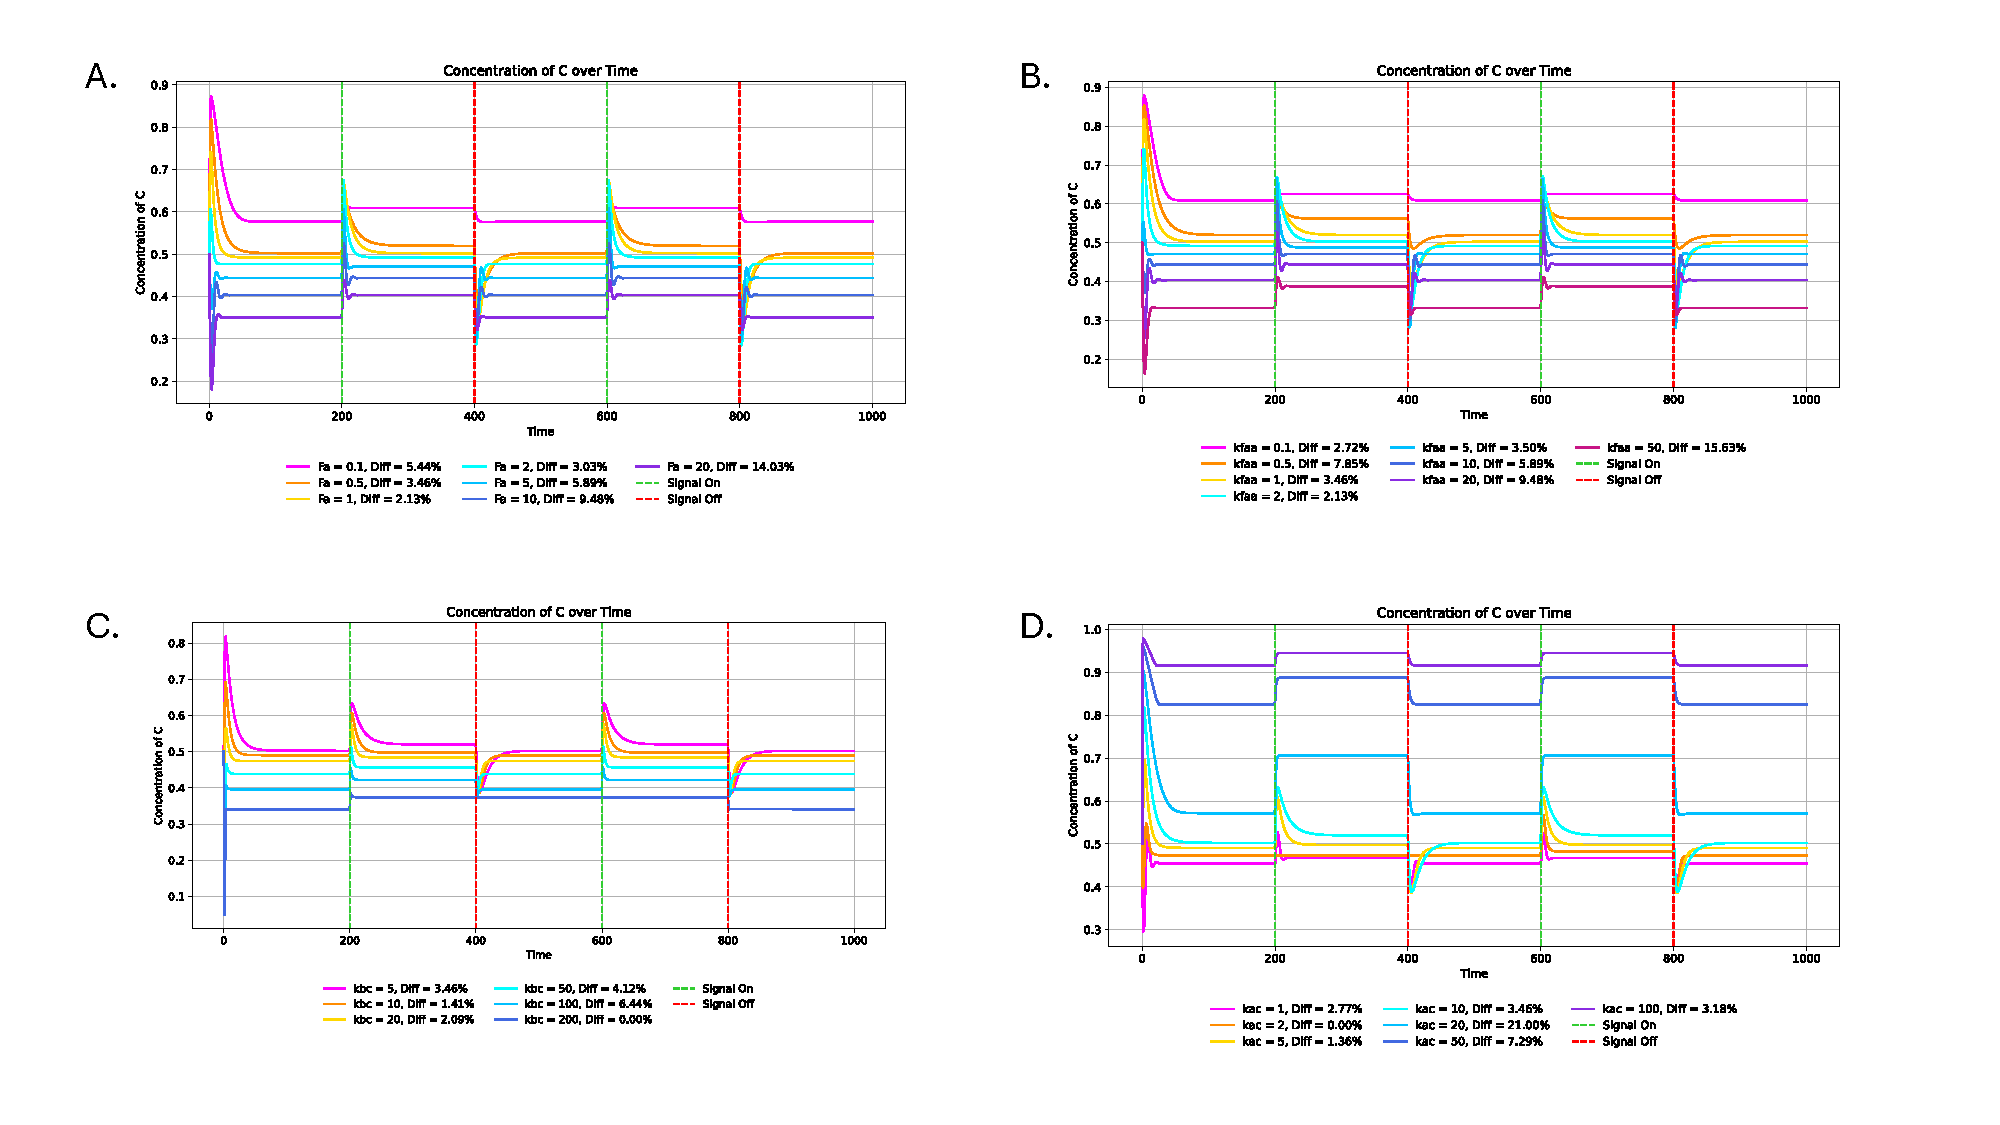
\includegraphics[width=0.7\textwidth]{/Users/olivia/Documents/Fall 2024/MCB 580/MCB580_Challenge2/report/negative_feedback_plus_D_explore_2.pdf}
    \caption{The NFLBN + \textit{D} shows improved robustness to changes in parameters \textit{Fa}, \textit{kfaa}, and \textit{kbc} compared to the NFLBN. It also shows limited robustness to changes in \textit{kac}. Varrying values for \textit{Fa} (A), \textit{kfaa} (B), \textit{kcb} (C) and \textit{kac} (D), with all other parameters set to the adaptive paramater values previously described. Input signal begins at 1, changes to 2 at the green dotted line, then goes back to 1 at the red dotted line. This continues every 200 time units. All other parameters held constant.}
    \label{fig:10}
\end{figure}

\begin{figure}[H]
    \centering
    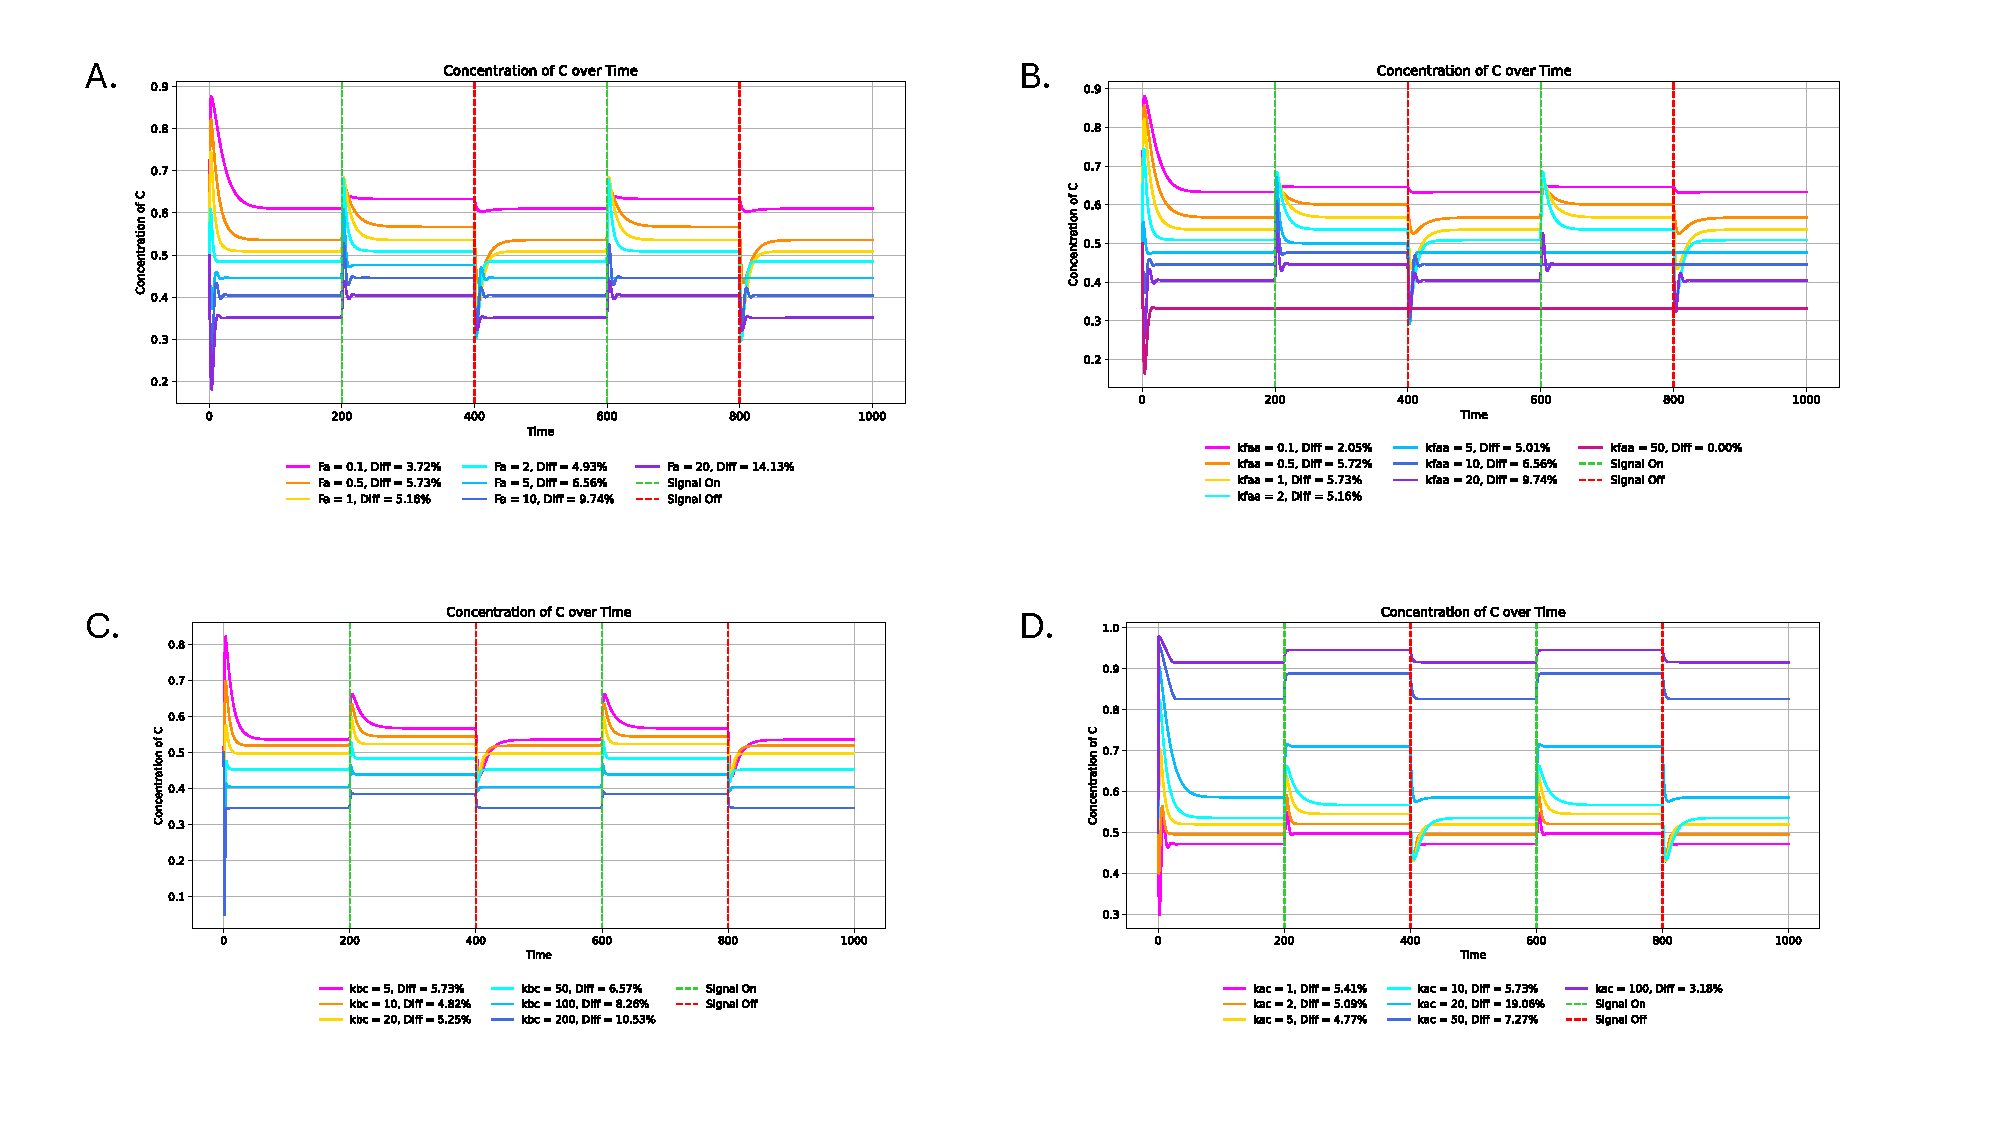
\includegraphics[width=0.7\textwidth]{/Users/olivia/Documents/Fall 2024/MCB 580/MCB580_Challenge2/report/negative_feedback_plus_D_plus_A_regulates_B_explore.pdf}
    \caption{The NFLBN + \textit{D} + \textit{A} regulates \textit{B} shows improved robustness to changes in parameters \textit{Fa}, \textit{kfaa}, \textit{kbc}, and \textit{kac} compared to the NFLBN. Robustness to change in \textit{Fa}, \textit{kfaa}, and \textit{kbc} values is seen in NFLBN + \textit{D}, but not robustness to changes in \textit{kac}. Varrying values for \textit{Fa} (A), \textit{kfaa} (B), and \textit{kcb} (C), and \textit{kac} (D), with all other parameters set to the adaptive paramater values previously described. Input signal begins at 1, changes to 2 at the green dotted line, then goes back to 1 at the red dotted line. This continues every 200 time units. All other parameters held constant.}
    \label{fig:11}
\end{figure}

\section{Discussion}

In this paper, we have shown that there is a set of parameters under which the negative feedback loop with a buffer node described in Ma et al. and shown in Figure 1 is adaptive \cite{challenge2paperD2L}. These parameter values are summarized in Table 1 and the behavior of the circuit in these conditions is seen in Figure 5. With this as a baseline, we sought to model a circuit that was similar in adaptive behavior but more robust to changes in parameter values. We explored to new circuits (Figure 2 and 3) where we added an additional node, \textit{D}, and added a direct relationship where \textit{A} regulates \textit{B}. Our first model, NFLBN + \textit{D}, shows robustness to changes in parameters \textit{Fa}, \textit{kfaa}, and \textit{kbc} while still responding adaptively, which we did not see in the simple NFLBN model. In the NFLBN + \textit{D} + \textit{A} regulates \textit{B} model, we continue to see robustness to changes in \textit{Fa}, \textit{kfaa}, and \textit{kbc} and also find robustness to changes in \textit{kac}, which we did not see in the NFLBN model or the NFLBN + \textit{D} model. In summary, we developed two models of adaptive circuits that are robust to changes in parameter values for specific parameters and still display the adaptive behavior of the simple negative feedback loop with a buffer node presented in Ma et al. \cite{challenge2paperD2L}. 

It is important to understand what features in a biochemical circuit increase robustness because having circuits that are robust to changes and can still behave as intended is biologically crucial. A biological system will undergo many perturbations and needs to be able to return to it's original state after those perturbations. Here, we have described the perturbation to be a change in the signal and the return to the original state as adaptive behavior, which we sought to find in the face of changing paramater values. Some examples of this phenomenon of a robust circuit design that occur naturally in biology are the system in bacteria responsible for chemotaxis \cite{chemotaxis}, the human immune system that can respond to a wide variety of pathogens under many different conditions \cite{immune}, and the ability of bacterial gene networks to still function despite changes in network connections \cite{gene}. In this paper, we explored a differnt type of network, one responsible for biochemical signaling, and found that specific network topologies are robust to changes in parameter values and can still display their adaptive behavior. 

\begin{thebibliography}{9}

\bibitem{challenge2paperD2L} 
Ma, W., Trusina, A., El-Samad, H., Lim, W. A., & Tang, C. (2009). Defining network topologies that can achieve biochemical adaptation. \textit{Cell}, 138(4), 760–773. https://doi.org/10.1016/j.cell.2009.06.013

\bibitem{chemotaxis} 
Alon, U., Surette, M., Barkai, N., & Leibler, S. (1999). Robustness in bacterial chemotaxis. \textit{Nature}, 397, 168–171. https://doi.org/10.1038/16483

\bibitem{immune} 
Wong, H. S., & Germain, R. N. (2018). Robust control of the adaptive immune system. \textit{Seminars in Immunology}, 36, 17–27. https://doi.org/10.1016/j.smim.2017.12.009

\bibitem{gene} 
Isalan, M., Lemerle, C., Michalodimitrakis, K., Horn, C., Beltrao, P., Raineri, E., Garriga-Canut, M., & Serrano, L. (2008). Evolvability and hierarchy in rewired bacterial gene networks. \textit{Nature}, 452(7189), 840–845. https://doi.org/10.1038/nature06847

‌

\end{thebibliography}

\end{document}